% Standalone submission-preparation draft. Compile from the repository root.
% The venue, authors, affiliations, funding, and corresponding author must be
% agreed with the supervisor before submission; no details are invented here.
\documentclass[11pt,a4paper]{article}
\usepackage[T1]{fontenc}
\usepackage[utf8]{inputenc}
\usepackage[english]{babel}
\usepackage[a4paper,margin=2.5cm]{geometry}
\setlength{\emergencystretch}{1em}
\usepackage{amsmath,amssymb,amsthm,booktabs,array}
\renewcommand{\qedsymbol}{\textnormal{QED}}
\usepackage{graphicx,float,hyperref}
\usepackage{placeins}
\usepackage[font=small,labelfont=bf]{caption}
\hypersetup{colorlinks=true,linkcolor=blue,citecolor=blue,urlcolor=blue}
\newtheorem{definition}{Definition}[section]
\newtheorem{proposition}{Proposition}[section]
\newtheorem{remark}{Remark}[section]
\newcommand{\OPT}{\texttt{OPT}}
\newcommand{\FEAS}{\texttt{FEASIBLE}}
\newcommand{\tablenote}[1]{\par\vspace{3pt}\begin{minipage}{\linewidth}\footnotesize\raggedright\textit{Note.} #1\end{minipage}\par}
\newcommand{\TreeGraphCount}{50}
\newcommand{\TreeObservationCount}{100}
\newcommand{\TreeTightCount}{48}

\newcommand{\ProgressObservations}{702}
\newcommand{\ProgressInstances}{117}
\newcommand{\ProgressJointStable}{74}
\newcommand{\ProgressOpen}{21}
\newcommand{\ProgressOpenPairs}{63}
\newcommand{\ProgressOpenSATUB}{39}
\newcommand{\ProgressOpenILPUB}{18}
\newcommand{\ProgressOpenEqualUB}{6}
\newcommand{\ProgressOpenILPLB}{13}
\newcommand{\ProgressOpenEqualLB}{50}
\newcommand{\ProgressMaxUB}{21}
\newcommand{\ProgressMaxLB}{24}
\newcommand{\ProgressSATOpt}{232}
\newcommand{\ProgressSATStable}{77}
\newcommand{\ProgressSATFeasible}{119}
\newcommand{\ProgressSATImprovedUB}{60}
\newcommand{\ProgressILPOpt}{281}
\newcommand{\ProgressILPStable}{91}
\newcommand{\ProgressILPFeasible}{70}
\newcommand{\ProgressILPImprovedUB}{68}
\newcommand{\ProgressReturnedFeasible}{1}
\newcommand{\ProgressClosed}{96}

\newcommand{\ProgressReportDir}{paper/generated/progress_confirmation/4927a34577a0c9d4}

% Generated by scripts/export_evidence_summary.py
\newcommand{\EvidenceInstances}{117}
\newcommand{\EvidenceTheory}{61}
\newcommand{\EvidenceOtherClosed}{35}
\newcommand{\EvidenceOpenBefore}{21}
\newcommand{\EvidenceCliqueCertified}{50}
\newcommand{\EvidenceNewlyClosed}{2}
\newcommand{\EvidenceClosedAfter}{98}
\newcommand{\EvidenceOpenAfter}{19}
\newcommand{\EvidenceVOneSame}{117}

\newcommand{\EvidenceReportDir}{results/analysis/evidence_summary/0700e674e1e6ba4e}

% Generated by scripts/analyze_color_order.py --publish
\newcommand{\ConstructionInstances}{117}
\newcommand{\ConstructionClosed}{101}
\newcommand{\ConstructionOpen}{16}
\newcommand{\ConstructionNewlyClosed}{3}
\newcommand{\ConstructionImproved}{3}
\newcommand{\ConstructionCliqueCertified}{53}
\newcommand{\ConstructionTotalNewlyClosed}{5}
\newcommand{\ConstructionCandidates}{113}
\newcommand{\ConstructionUnknown}{4}

\newcommand{\ConstructionReportDir}{results/analysis/color_order/2d62af353a1756ae}

% Generated by scripts/export_submission_tables.py
\newcommand{\SubmissionSummaryDir}{paper/generated/submission_summary/af1f510739b1e214}
\newcommand{\SupportInstances}{117}
\newcommand{\SupportTheory}{61}
\newcommand{\SupportClique}{53}
\newcommand{\SupportOverlap}{24}
\newcommand{\SupportIndependent}{90}
\newcommand{\SupportSolverDependent}{11}
\newcommand{\SupportClosed}{101}
\newcommand{\SupportOpen}{16}


\title{SAT-Based Approach for\\$L(h,k)$-Labeling of General Graphs}
\author{}
\date{October 18, 2026}

\begin{document}
\maketitle
\begin{abstract}
We study an exact SAT approach to minimum-span $L(h,k)$-labeling of
simple undirected graphs with $h\geq k\geq1$. An order encoding and
bounded span search are proved correct and compared with assignment
integer linear programming (ILP). On 117 tree, grid and random-graph
instances, with three repetitions and a 30-second limit, SAT and ILP
prove optimality in every repetition on \ProgressSATStable{} and
\ProgressILPStable{} instances, respectively. ILP has greater optimality
coverage, while feasible upper bounds favor different backends on some
instances unresolved within the time limit.
Supplementary clique and weighted-capacity bounds, explicit labelings,
and proof-producing SAT search independently certify all 117 optima.
The final evidence comprises 91 theory/clique certificates, 15
weighted-capacity certificates and 11 replayed UNSAT proofs; it does not
change the original timed coverage.
A separate $L(2,1)$ symmetry study reports 494 jointly optimal pairs
out of 496. Cycles show a median clause reduction of 12.58\%, with
little change in the median time ratio; effects vary across product
families. The results distinguish model size, feasible-solution quality
and proof coverage, while documenting the limits of the evaluated methods.
\end{abstract}
\noindent\textbf{Keywords:} $L(h,k)$-labeling, SAT, order encoding,
exact optimization, ILP, optimality certificates.

\section{Introduction}
The $L(h,k)$-labeling problem assigns nonnegative integers to graph
vertices, with prescribed separation at distances one and two. It
originates in frequency assignment, where nearby transmitters require
different levels of interference protection \cite{griggs,calamoneri}.
The objective is to minimize the span between the largest and smallest
labels. Formulas are known for particular graph classes and parameter
regimes; a general-purpose exact method must also handle inputs for which
these formulas do not determine the optimum.

This study develops and evaluates an exact SAT pipeline for finite simple
undirected graphs with $h\geq k\geq1$. Boolean threshold variables encode
labels, and a bounded span search maintains a feasible solution together
with a lower bound. Assignment integer linear programming (ILP) provides
the principal exact baseline. Both methods can prove optimality, but may
retain an open interval when their time budget expires. We therefore
compare feasible-solution quality and proof coverage alongside runtime.
``General graphs'' describes the formulation's input domain, not a claim
of efficient solution on every graph.

Four research questions organize the study:
\begin{enumerate}
\item\label{rq:correctness} Does the SAT encoding preserve feasibility,
and does the span search report optimality only when it is established?
\item\label{rq:theory} Where exact formulas or proven bounds apply, do
computed labelings agree with them, and which instances can be certified
by matching lower and upper bounds?
\item\label{rq:comparison} How do runtime, model size and optimality
coverage compare between SAT and assignment ILP across the evaluated
graph sizes and families?
\item\label{rq:symmetry} For families with justified symmetries, how do
symmetry-breaking constraints affect CNF size and solution time?
\end{enumerate}

The study makes four contributions:
\begin{enumerate}
\item A general-graph SAT pipeline with encoding equivalence, a
span-search invariant and justified symmetry conditions.
\item Independent labeling checks and reference-bound comparisons,
with retained graphs, configurations and witnesses for reproducibility.
\item A comparison with assignment ILP on 117 fixed graph/parameter
instances that reports unresolved cases, bound quality and proof
coverage alongside runtime. A separate paired $L(2,1)$ study evaluates
symmetry effects by family under its original backend and budget.
\item A supplementary certificate pipeline combining mathematical
bounds, explicit labelings and independently replayed UNSAT proofs.
Clique and color-order certificates first close five of the 21 intervals
left open by pooled solver evidence. Weighted capacity bounds and a
color-rank-residual SAT formulation then close the remaining 16, yielding
independently checked optimal spans for all 117 instances.
\end{enumerate}

SAT and ILP formulations for distance-constrained labeling already exist
\cite{shao2013distance,shao2014strong}, and order encoding is established
\cite{tamura2009order}. Our contribution is the verified formulation and
the accompanying evidence on exact search, bound quality and symmetry
effects under stated protocols. The computational certificates establish
optima for the evaluated instances; they do not establish new formulas
over entire graph families.

\section{Preliminaries and related work}
\subsection{Definitions and conventions}
Let $G=(V,E)$ be a finite simple undirected graph, and let
$D_2=\{\{u,v\}:d_G(u,v)=2\}$ contain unordered vertex pairs at shortest-path
distance exactly two. For integers $h\geq k\geq1$, a labeling
$f:V\to\mathbb Z_{\geq0}$ satisfies
\[
 |f(u)-f(v)|\geq h\quad(\{u,v\}\in E),\qquad
 |f(u)-f(v)|\geq k\quad(\{u,v\}\in D_2).
\]
Its span is $\max_v f(v)-\min_v f(v)$; the minimum span is
$\lambda_{h,k}(G)$. Translating the minimum label to zero preserves every
constraint. Thus a decision test for span at most $s$ uses labels
$0,\ldots,s$, with $s+1$ available values. Vertices farther than two apart
may share a label. Disconnected components impose no constraints on one
another, and their optimal spans combine by taking the maximum. An empty
or edgeless graph has span zero.


For a nonempty graph, its square $G^2$ joins vertices at distance one or
two in $G$. In particular,
\[
 \lambda_{1,1}(G)=\chi(G^2)-1.
\]
A proper coloring with $q$ colors yields labels $0,\ldots,q-1$;
conversely, integer labels of span $s$ use at most $s+1$ colors of $G^2$.
This connects the equal-parameter case to coloring without identifying
arbitrary $L(h,k)$ instances with ordinary coloring.

We write $P_n,C_n$ for paths and cycles. The Cartesian product
$G\square H$ has vertices $(u,v)$; an edge changes exactly one coordinate
along an edge of that factor. The corona $G\circ H$ attaches a separate
copy of $H$ to every vertex of $G$, adjacent to all vertices in its copy.
For $|V(G)|=n$ and $|V(H)|=m$, the corona has $n(m+1)$ vertices.
Figure~\ref{fig:submission-labeling} illustrates labels and thresholds.

\begin{figure}[htbp]
\centering
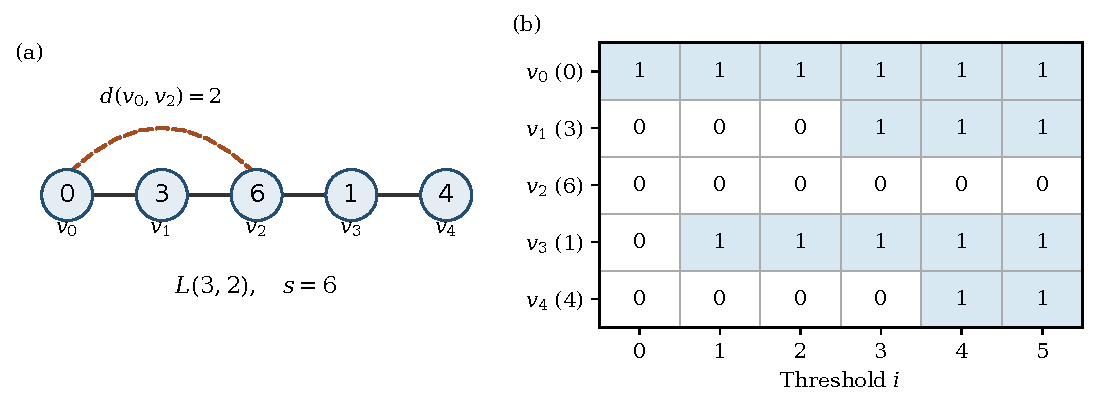
\includegraphics[width=\linewidth]{paper/generated/manuscript_figures/labeling_order.pdf}
\caption{A labeling and its threshold representation.}
\label{fig:submission-labeling}
\tablenote{The labels $0,3,6,1,4$ on $P_5$ satisfy $L(3,2)$ and have
span 6. The dashed arc indicates a distance-two pair, not an edge.
Threshold cells represent $[f(v)\leq i]$; the boundary at $i=6$ is constant.}
\end{figure}

\subsection{Related work}
Griggs and Yeh developed foundational results for $L(2,1)$-labeling
\cite{griggs}; Calamoneri surveys $L(h,k)$-labeling across graph classes
and parameter regimes \cite{calamoneri}. These results provide both
motivation and reference values for computational methods. Specialized
algorithms can exploit structure: $L(2,1)$-labeling on trees admits a
linear-time algorithm \cite{hasunuma}, whereas the tree complexity
result of Fiala, Golovach and Kratochv\'il includes the nondivisible
parameter regime represented here by $(3,2)$ \cite{fiala2008trees}.
Worst-case hardness does not imply that each sampled tree is difficult.
Murugan studied $L(2,1)$-labeling of corona products
\cite{murugan2015corona}; these families are established objects of study,
not new labeling classes introduced by this experiment. Work on structural
parameters motivates reporting graph structure alongside vertex count
\cite{fiala2018parameterized}; its parameterized algorithm is not evaluated here.

Exact SAT and ILP approaches precede this study. Shao and Vesel presented
assignment ILP and direct SAT formulations for distance-constrained
$L(k_1,\ldots,k_r)$-labeling, with experiments on $L(3,2,1)$
\cite{shao2013distance}. Their $L(2,1)$ work used direct SAT encoding on
strong products \cite{shao2014strong}. Tamura et al.\ describe the
order encoding of finite-domain comparisons using threshold variables
\cite{tamura2009order}. We use this representation for two configurable
distance constraints and evaluate the resulting implementation against
assignment ILP on common instances. The cited implementations have not
been reproduced under our protocol, so no performance ranking against
them is inferred.

Related variants provide context rather than interchangeable benchmark
values. Edge labeling corresponds to vertex labeling on a line graph,
subject to its distance convention \cite{berthe2023edge};
$L(h,1,1)$-labeling also constrains distance three \cite{king2010trees}.
Neither is the present two-distance model. The radio-labeling
preprint by Vu Thanh et al.\ uses order encoding and incremental SAT
\cite{vu2026radio}, while Sarhan et al.\ study a genetic algorithm for
radio labeling \cite{sarhan2026genetic}. Radio labeling with parameter
$r$ requires separation $r+1-d(u,v)$: $r=2$ gives $L(2,1)$, but $r=3$
also constrains distance three and therefore differs from $L(3,2)$.
Their numerical results are not reference values for our general
two-distance problem. An adapted genetic algorithm remains a possible
feasible-solution baseline and is not evaluated here.

Theoretical bounds, heuristic constructions and exact solvers provide
complementary evidence. A feasible labeling gives an upper bound; a
matching proven lower bound certifies optimality, regardless of how the
labeling was found. Otherwise, an exact solver must exclude smaller
spans to close the interval. This distinction underlies our separate
reporting of timed solver outcomes and combinatorial certificates.

\section{SAT-based method}
\label{sec:submission-method}
\subsection{Order encoding and correctness (RQ1)}
For each vertex, introduce $x_{v,i}\Leftrightarrow[f(v)\leq i]$ for
$0\leq i<s$, and use constants $x_{v,-1}=\bot$, $x_{v,s}=\top$.
The clauses
\begin{equation}
 \neg x_{v,i}\lor x_{v,i+1},\qquad 0\leq i<s-1,
\end{equation}
force monotonicity. Since $f(v)=a$ is equivalent to
$x_{v,a}\land\neg x_{v,a-1}$, a forbidden label pair $(a,b)$ is excluded by
\begin{equation}\label{eq:submission-forbidden}
 \neg x_{u,a}\lor x_{u,a-1}\lor\neg x_{v,b}\lor x_{v,b-1}.
\end{equation}
Generate this clause for $|a-b|<h$ on edges and $|a-b|<k$ on $D_2$,
with $0\leq a,b\leq s$, simplifying boundary constants.
For $L(2,1)$ the unsimplified clause count is
\[
 |V|\max(s-1,0)+|E|A(s)+|D_2|(s+1),\qquad
 A(s)=\begin{cases}1,&s=0,\\3s+1,&s\geq1.\end{cases}
\]
General-parameter counts are given in Table~\ref{tab:submission-symbolic}.


\begin{proposition}\label{prop:submission-encoding}
The resulting CNF is satisfiable exactly when an $L(h,k)$-labeling of
span at most $s$ exists.
\end{proposition}
\begin{proof}
A labeling in $[0,s]$ supplies monotone threshold values and violates no
forbidden-pair clause. Conversely, each monotone threshold sequence
determines one label: the first true index, or $s$ if all variables are
false. A decoded violation falsifies its clause in
\eqref{eq:submission-forbidden}, so every decoded labeling is valid.
Translation establishes the statement for span rather than maximum label.
For $s=0$, any positive separation requirement produces an empty clause;
with no constrained pairs, the all-zero labeling is feasible.
\end{proof}

Implementation tests compare both search strategies with an exhaustive
oracle on all nonisomorphic graphs with at most five vertices for $L(2,1)$.
The generalized tests cover all such graphs up to four vertices for
$(1,1),(2,1),(3,2),(1,3),(0,2),(2,0),(0,0)$, using Glucose and CaDiCaL.
Assignment-level checks exhaust the eight three-vertex graphs with
$s=0,\ldots,4$ for $L(2,1)$, with additional $h,k$ checks on small graphs.
Separate tests check simplification equivalence, constructor reflections,
and assignment-ILP constraints. These finite tests support implementation
validation; the proposition establishes general equivalence.



\subsection{Bounds and span search}
For a graph with an edge, use $L=h+(\Delta-1)\min(h,k)$,
which is $h+(\Delta-1)k$ in the present domain. In the closed
neighborhood of a maximum-degree vertex, sorted labels have $\Delta$
gaps of at least $k$, at least one of which is incident to the center
and has size at least $h$. This proves the lower bound. A greedy labeling
chooses the smallest legal nonnegative label at each vertex in a fixed
order; its validated span supplies $U$.

The linear strategy tests $s=U-1$; the hybrid strategy used in the
benchmarks tests $s=\lfloor(L+U)/2\rfloor$. Each trial uses a fresh CNF
and solver. SAT supplies a validated labeling and reduces $U$ to its
actual span; UNSAT raises $L$ to $s+1$. Learned clauses are not reused
across trials. Figure~\ref{fig:submission-pipeline} summarizes the procedure.

\begin{proposition}\label{prop:submission-search}
Given valid initial bounds, an equivalent decision encoding and
satisfiability-preserving symmetry constraints, the span search reports
\OPT{} only for an optimal incumbent.
\end{proposition}
\begin{proof}
The invariant is $L\leq\lambda_{h,k}(G)\leq U$, with a labeling supporting
$U$. SAT preserves the upper inequality. UNSAT at $s$ excludes every
span at most $s$, preserving the lower inequality after $L=s+1$.
Equality $L=U$ proves optimality, including when the initial bounds meet.
An interrupted trial makes neither update and cannot be treated as UNSAT.
\end{proof}

\begin{figure}[htbp]
\centering
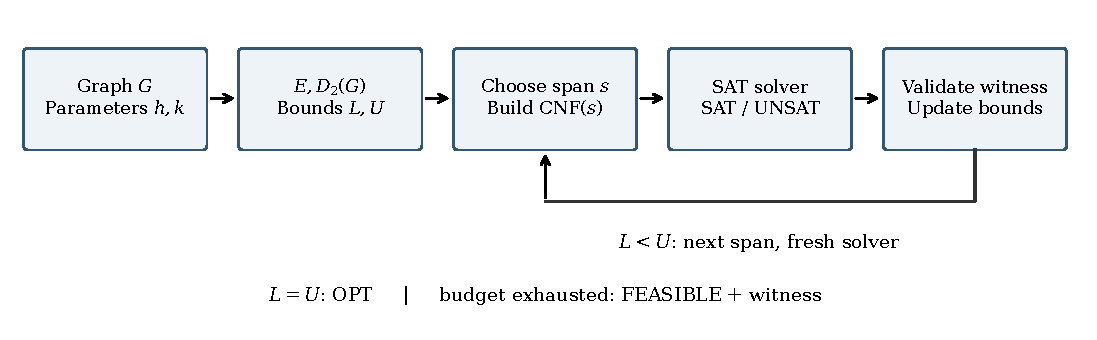
\includegraphics[width=\linewidth]{paper/generated/manuscript_figures/solver_pipeline.pdf}
\caption{Bounded SAT span search.}
\label{fig:submission-pipeline}
\tablenote{Only completed SAT or UNSAT decisions update the interval.
Timeout retains the last justified bounds and feasible labeling.}
\end{figure}

\subsection{Symmetry breaking}
\begin{proposition}\label{prop:submission-transitivity}
For a vertex-transitive graph, imposing $f(v_0)=0$ preserves the optimum
and feasibility of the decision problem with span at most $s$.
\end{proposition}
\begin{proof}
Translate a valid labeling so that some vertex $w$ has label zero.
An automorphism taking $v_0$ to $w$ preserves all distances; composing
the labeling with it assigns zero to $v_0$ without changing the span.
\end{proof}
Root fixing is used only for cycles in the symmetry experiment.
For $C_n$, choose $t$ attaining the minimum label and put
$g(i)=f((i+t)\bmod n)-f(t)$. Rotation and translation preserve feasibility
and span, so $g(0)=0$. Reflection about 0 then permits
$g(1)<g(n-1)$, since the two neighbors must have distinct labels.
Other tested families use only reflection orders: on $C_n\square H$,
$(i,j)\mapsto(-i\bmod n,j)$ exchanges $(1,0)$ and $(n-1,0)$;
on $C_n\circ H$, reflect the core and the attached copies together.
$H$ is a path or cycle. These automorphisms justify the selected order
without fixing a root. No additional constraint is used for
$P_n\square P_m$ or $P_n\circ H$.

Both configurations remove tautologies and duplicates and propagate
units to a fixed point. Fixed cycle-root thresholds are represented by
constants; retained unit clauses allow complete decoding. An order
constraint removes symmetric solutions, but may add clauses before
simplification. It does not guarantee halved CNF size or runtime.

\subsection{Combinatorial optimality certificates}
\begin{proposition}\label{prop:square-clique}
If $Q$ is a nonempty clique in the square $G^2$, then
$\lambda_{h,k}(G)\geq k(|Q|-1)$ for $h\geq k\geq1$.
A valid labeling attaining this bound is optimal.
\end{proposition}
\begin{proof}
Every pair in $Q$ is at distance one or two in $G$. Consecutive sorted
labels differ by at least $k$, and their $|Q|-1$ gaps sum to the bound.
A labeling attaining it supplies the matching upper bound.
\end{proof}
Any such clique suffices; it need not be proved maximum. The postprocessor
enumerates maximal cliques on the current small graphs and selects a
largest one, with lexicographic tie breaking. This potentially exponential
step is outside the timed solver comparison. A separate standard-library
checker verifies the original graph, clique membership and full labeling.
The following condition supplies additional witnesses.

\begin{proposition}[A sufficient color-order condition]
\label{prop:color-order}
Let $G$ be a nonempty simple undirected graph and $0<k\leq h\leq2k$.
Suppose $C_1,\ldots,C_r$ partition $V(G)$ into nonempty independent sets
of $G^2$. If $h>k$, suppose additionally that no edge of $G$ joins
consecutive classes $C_i,C_{i+1}$. Then
\[
 f(v)=k(i-1)\quad\text{for }v\in C_i
\]
is an $L(h,k)$-labeling of span $k(r-1)$.
If $G^2$ also contains a clique of size $r$, this span is optimal.
\end{proposition}
\begin{proof}
Vertices in the same class have distance greater than two, so equal
labels violate no constraint. Distinct classes have label difference at
least $k$, satisfying every distance-two constraint. If $h=k$, this also
suffices for edges. Otherwise, an edge cannot join consecutive classes
by assumption, and its endpoints differ by at least $2k\geq h$.
Every class is nonempty, so the span is $k(r-1)$. A square clique of size
$r$ gives the matching lower bound by Proposition~\ref{prop:square-clique}.
\end{proof}

\paragraph{Bounded construction.}
The implementation constructs a maximum-cardinality matching in the
complement of $G^2$. Each matched pair forms a class; unmatched vertices
form singleton classes. Every class is therefore independent in $G^2$.
This restricts the construction to classes of size at most two and need
not find a minimum coloring of $G^2$. Maximum matching only minimizes
the number of classes within this restricted partition scheme; its
optimality is unnecessary for checking a resulting labeling.

For $h>k$, define a compatibility graph on the classes, with an edge
between two classes exactly when no original graph edge joins them.
The required ordering is a Hamiltonian path in this compatibility graph.
A seeded insertion heuristic starts at a low-degree class, repeatedly
inserts an unplaced class into a compatible position, and restarts if
it cannot continue. It makes at most 100 attempts, with algorithmic seed 0
and canonical vertex and class ordering. The algorithmic seed is separate
from each archived graph-generation seed. A failure is reported as
\texttt{UNKNOWN}; it proves neither nonexistence of an ordering nor
infeasibility of the labeling instance. When $h=k$, no ordering search
is needed. Parameters outside the sufficient condition are not handled
by this construction; the general SAT/ILP formulations retain their
original domain.


The construction was developed after examining the unresolved instances.
Its subsequent whole-cohort application records both successes and
failures, but is not a held-out performance evaluation.


\subsection{Assignment ILP baseline}
Given a validated greedy upper bound $U$, let $y_{v,a}=1$ select label
$a\in\{0,\ldots,U\}$. The baseline minimizes $\ell_{\max}$ subject to
\begin{align}
 \sum_{a=0}^{U}y_{v,a}&=1 &&(v\in V),\\
 y_{u,a}+y_{v,b}&\leq1 &&(\{u,v\}\in E,\ |a-b|<h),\\
 y_{u,a}+y_{v,b}&\leq1 &&(\{u,v\}\in D_2,\ |a-b|<k),\\
 \sum_{a=0}^{U}a\,y_{v,a}&\leq\ell_{\max} &&(v\in V),\\
 y_{v,a}&\in\{0,1\},\qquad \ell_{\max}\in\{0,\ldots,U\}.
\end{align}
Exactly one label is chosen at each vertex, and all violating pairs are
forbidden. Every valid labeling in this domain supplies a feasible
assignment. Translation invariance therefore makes minimizing the maximum
label equivalent to minimizing span; no arbitrary vertex is fixed to zero.

To compare representation sizes, use a common domain $[0,s]$, set
$n=|V|$, and define
\[
 t_d=\min(s,d-1),\quad
 F(s,d)=(s+1)(2t_d+1)-t_d(t_d+1),\quad
 B=|E|F(s,h)+|D_2|F(s,k).
\]
Here $F(s,d)$ counts ordered label pairs with difference less than $d$.
Table~\ref{tab:submission-symbolic} gives the model sizes before
symmetry breaking or simplification.
\begin{table}[htbp]
\centering\small
\caption{Symbolic model sizes at span $s$.}
\label{tab:submission-symbolic}
\begin{tabular}{lll}
\toprule
Model & Variables & Clauses/rows\\\midrule
Order SAT & $ns$ & $n\max(s-1,0)+B$\\
Direct SAT (pairwise AMO) & $n(s+1)$ & $n(1+\binom{s+1}{2})+B$\\
Assignment ILP & $n(s+1)+1$ & $2n+B$\\
\bottomrule
\end{tabular}
\tablenote{Raw counts without symmetry breaking or preprocessing;
AMO means at most one. ILP includes one integer maximum-label variable;
variable bounds are not counted as rows.}
\end{table}
Direct SAT forbids a label pair with two literals, versus at most four
in order encoding. Other AMO encodings can alter the direct model size.
These are representation
counts, not equal-cost operations or a runtime ranking. Enumerating only
forbidden pairs costs $O((s+1)\min(s+1,2d-1))$ per constrained vertex
pair; this does not bound the complexity of solving the resulting model.


Under a one-based domain $1,\ldots,U'$, the optimal maximum label is
$\lambda_{h,k}+1$ for a nonempty graph. Our zero-based convention avoids
that offset. A Big-M formulation is also implemented: each separated
pair uses an orientation binary and two inequalities, with
$M=U+\max(h,k)$. It is not the baseline in the primary experiment;
no result here ranks all ILP formulations.

\section{Experimental evaluation}
\label{sec:submission-results}
\subsection{Cohort and protocol}
The primary experiment uses a fixed cohort of 39 graphs. Each graph is
evaluated with $(h,k)=(1,1)$, $(2,1)$ and $(3,2)$, giving 117 labeling instances.
It comprises nine random labeled trees with 20, 40 and 60 vertices and
three graph-generation seeds per size; three grids
$P_4\square P_5$, $P_5\square P_8$ and $P_6\square P_{10}$;
18 Erd\H{o}s--R\'enyi graphs with the same sizes and seeds and edge
probabilities $p\in\{0.15,0.30\}$; and nine Barab\'asi--Albert graphs
with the same sizes and seeds and attachment parameter $m=2$.
Disconnected samples are retained. The graph cohort is not reselected
according to solver outcomes.

The SAT backend is CaDiCaL with order encoding and a fresh solver for each
span trial. The ILP baseline is Gurobi with the assignment formulation,
one thread and a greedy MIP start. Symmetry breaking is disabled in this
comparison. Each instance has three repetitions per backend, producing
\ProgressObservations{} observations. Backends run sequentially in
separate processes, with their order rotated across instances and
repetitions. Each run has a 30-second external limit; elapsed wall time
includes startup, model construction, solving and cleanup. Parent-side
witness validation is outside the recorded worker interval.
The shared comparison runner's external deadline governs both backends;
the individual solver APIs' time-limit mechanisms are not assumed equivalent.

The completed \texttt{isolated-progress-v2} run retains intermediate
validated incumbents and lower-bound updates. SAT transmits completed
span decisions; Gurobi transmits available incumbent and bound information.
A timeout without a closed interval is reported as \FEAS, not \OPT.
One Gurobi observation returned \FEAS{} early; its native stopping reason
was not recorded, so it remains a feasible observation with an unknown
native termination reason. No \OPT{} observation exceeds the recorded budget.

The source manifest, explicit graphs, configurations, bounds and saved
labelings are retained with the raw results. An audit checks all
\ProgressObservations{} witnesses and the expected cohort and repetitions.
Label validation independently checks shortest-path constraints, but does
not verify SAT UNSAT traces or MILP dual certificates. Historical pilot,
v1 and supplementary $L(2,1)$ symmetry results remain in the companion
research report and archive; their timings are not pooled into this experiment.

\subsection{Optimality coverage and bound quality}
\begin{table}[htbp]
\centering\small
\caption{Optimality coverage within 30 seconds.}
\label{tab:submission-coverage}
\input{\ProgressReportDir/coverage.tex}
\tablenote{Each backend has 351 observations on 117 instances. All-three OPT
counts instances proved optimal in every repetition. Improved UB counts
FEASIBLE observations with a saved feasible span smaller than the shared
initial incumbent. It does not establish optimality.}
\end{table}

Table~\ref{tab:submission-coverage} shows more stable optimality proofs for
Gurobi: \ProgressILPStable/117 instances, compared with
\ProgressSATStable/117 for CaDiCaL. Both backends are optimal in all three
repetitions on \ProgressJointStable{} instances. Repetitions are observations
of the same graphs, not additional independent graph samples. Runtime
comparisons restricted to this common solved subset would need to be read
alongside the coverage difference; they cannot characterize unsolved instances.

\begin{table}[htbp]
\centering\small
\caption{Paired lower- and upper-bound comparisons.}
\label{tab:submission-bounds}
\input{\ProgressReportDir/bounds.tex}
\tablenote{Pairs match the same graph, parameter pair and repetition. A
higher lower bound and a smaller validated upper bound are preferable.
The open subset comprises the 21 instances unresolved after pooling v2
solver evidence, before either combinatorial postprocessing step. Its
63 pairs are retained as a fixed analysis subset; they are not the final
\ConstructionOpen{} open instances in Table~\ref{tab:submission-evidence}.}
\end{table}

On this initially open subset, SAT has a smaller feasible upper bound in
\ProgressOpenSATUB{} pairs, ILP in \ProgressOpenILPUB{}, and
\ProgressOpenEqualUB{} tie. ILP has a stronger recorded lower bound in
\ProgressOpenILPLB{} pairs and \ProgressOpenEqualLB{} tie; SAT has none
with a stronger lower bound on this subset. These outcomes distinguish
solution quality from the ability to exclude smaller spans. They support
complementary behavior on the measured instances, not equivalent
effectiveness or universal dominance by either method.

\subsection{Consolidated optimality evidence}
\begin{table}[htbp]
\centering\small
\caption{Consolidated instance-level evidence.}
\label{tab:submission-evidence}
\input{\ConstructionReportDir/summary.tex}
\tablenote{Original-v2 columns: Theory denotes a witness attaining the
applicable initial theoretical bound; Other denotes additional closed
intervals. Theory + Other + Open = Cases. The final columns include both
certification steps: two new closures from cliques with stored witnesses
and three from color-order constructions. Clique-cert. counts matching
square-clique bounds and labelings; it overlaps Closed and is not added
again. Closed + Open = Cases. Counts are distinct graph/parameter
instances, not per-run successes; timed solver coverage remains unchanged.}
\end{table}

Applicable formulas and bounds provide a separate correctness reference.
In particular, the equal-parameter tree formula and the $L(2,1)$ grid
formula in the appendix cover 12 instances in this cohort. References
are used only within their stated graph and parameter domains. Agreement
on tested instances is validation evidence, rather than a proof of a new
formula over an entire family.

Pooling v2 solver intervals originally closed \ProgressClosed{} instances.
The square-clique analysis increased this to \EvidenceClosedAfter{} by
matching a lower bound to stored feasible witnesses in two previously
unresolved cases. The additional construction in
Section~\ref{sec:color-order-results} supplies new explicit witnesses and
closes \ConstructionNewlyClosed{} more. Table~\ref{tab:submission-evidence}
is the final instance-level summary. Solver-dependent proofs remain
distinguished from directly checked combinatorial certificates.

A separate screen of \TreeGraphCount{} $L(3,2)$ trees with 100--1600 vertices
found matching reported optimal spans for both backends; \TreeTightCount{}
attain the degree bound. Its different size range, single run per graph
and backend, and 60-second limit prevent pooling its timings with the
primary experiment. It supplies additional structured-graph validation,
not evidence that every tree is easy or that the degree bound is always tight.

\subsection{Validity and reproducibility limits}
The cohort includes several graph models but only three graph-generation
seeds at each randomized configuration and 20--60 vertices in the primary
comparison. Its observations do not represent all graphs or all solver
implementations. Assignment ILP is one formulation; the results are not a
comparison with every possible ILP method. SAT/ILP agreement supplements,
but does not replace, mathematical arguments or independent certificates.

The experiment does not include a controlled direct-versus-order encoding
ablation, incremental SAT or a GA baseline. Clause counts measure model
representation and do not prove runtime improvements. The post-hoc
construction is analyzed separately from timed solver performance.
Historical hardware metadata are incomplete, so no reference-machine
performance claim is inferred from the available software versions alone.

Raw observations, witnesses and manifests remain under \path{results/runs/}.
The v2 analysis, combinatorial certificates and consolidated summaries are
stored in versioned directories under \path{results/analysis/}. Source
fingerprints link derived tables to their inputs. The report-generation
targets revalidate saved evidence and compile the manuscript without
rerunning the original solver experiment.

\section{Conclusion}
We developed an exact SAT pipeline for minimum-span $L(h,k)$-labeling,
established the correctness of its encoding and span search, and evaluated
it against assignment ILP on a fixed multi-family cohort. In the repeated
30-second comparison, SAT and ILP establish optimality in all three runs
on \ProgressSATStable{} and \ProgressILPStable{} of 117 instances,
respectively. The remaining-bound analysis shows why feasible-solution
quality and optimality proofs must be evaluated separately.

Combinatorial postprocessing complements this comparison. Combining the
existing evidence with verified square-clique bounds and explicit
color-class ordering witnesses closes \ConstructionClosed{} instances
and leaves \ConstructionOpen{} open. Of the closed instances,
\ConstructionCliqueCertified{} have matching square-clique bounds and
labelings, allowing a solver-independent optimality check. These
certificates concern the evaluated instances and are not additional
timed solver successes or a new exact formula for an entire graph class.

The contribution is a correct general-graph formulation with an auditable
comparison of exact methods and explicit limits of their current evidence.
The study does not claim that order encoding is new or that SAT dominates
ILP. A controlled encoding ablation and independently checkable UNSAT
traces are possible future extensions. Resolving every remaining interval
is not required to report the established results and computational limits
of the present experiment.


\begingroup
\small
\bibliographystyle{plain}
\bibliography{paper/references}
\endgroup
\clearpage
\appendix
\section{Proven reference bounds}
The following results validate the formulations and are not claimed as new
contributions to graph classification. Labeling of Cartesian-product classes
has already been studied \cite{calamoneri}. Complete proofs are included
to avoid inferring formulas over infinite families from finite observations.

\begin{proposition}\label{prop:equal-tree}
For a nonempty tree $T$ and integer $h=k\geq1$,
$\lambda_{h,h}(T)=h\Delta(T)$.
\end{proposition}
\begin{proof}
The closed neighborhood of a degree-$\Delta$ vertex contains $\Delta+1$
vertices at pairwise distance at most 2, requiring span at least $h\Delta$.
For the upper bound, root the tree and color its square with $\Delta+1$
colors, level by level. Assign distinct colors to the children of each
vertex, excluding the colors of that vertex and its parent, if present.
A non-root vertex has at most $\Delta-1$ children and at least $\Delta-1$
available colors; the root has at most $\Delta$ children and $\Delta$
available colors. Distance-1 or distance-2 pairs are parent--child,
grandparent--grandchild, or sibling pairs, so this coloring is valid.
Multiplying colors $0,\ldots,\Delta$ by $h$ gives a labeling attaining
the bound. A one-vertex tree has span 0 and also satisfies the formula.
\end{proof}

For any graph with $n\geq1$ vertices, assigning distinct labels
$0,q,\ldots,(n-1)q$, where $q=\max(h,k)$, gives the elementary upper bound
$\lambda_{h,k}\leq(n-1)q$. This bound can be loose and differs from the
upper bound supplied by a specific heuristic labeling. In the comparisons,
the degree bound $h+(\Delta-1)\min(h,k)$ is also recorded separately
from final solver bounds.

\begin{proposition}\label{prop:extreme}
In an $L(2,1)$-labeling using labels $0,\ldots,\Delta+1$, every vertex
of degree $\Delta$ must receive label 0 or $\Delta+1$.
\end{proposition}
\begin{proof}
Its neighbors require $\Delta$ distinct labels because each pair is adjacent
or at distance 2. If the central label is $a\in\{1,\ldots,\Delta\}$,
labels $a-1,a,a+1$ are forbidden on its neighbors. Only $\Delta-1$ labels
remain, which is insufficient. The central label must therefore be a domain endpoint.
\end{proof}

\begin{proposition}\label{prop:grid}
For $n,m\geq4$, $\lambda_{2,1}(P_n\square P_m)=6$.
\end{proposition}
\begin{proof}
Index coordinates from 0 and define $f(i,j)=(2i+3j)\bmod7$, with
representatives in $\{0,\ldots,6\}$. Across an edge, the label difference
modulo 7 is $\pm2$ or $\pm3$, so the absolute difference between
representatives is at least 2. At distance 2, coordinate displacements are
$(\pm2,0),(0,\pm2),(\pm1,\pm1)$; the differences modulo 7 belong to
$\{\pm4,\pm6,\pm1,\pm5\}$ and are nonzero. This gives a valid labeling
of span at most 6.

Suppose a labeling has span at most 5 and translate it into $0,\ldots,5$.
The three internal vertices $(1,1),(1,2),(2,2)$ all have degree 4.
Proposition~\ref{prop:extreme} restricts them to labels 0 and 5. The two
successive edges force alternating labels, giving equal labels to the
endpoints. Their distance is 2, a contradiction. Thus the span is at least 6.
\end{proof}
The bound $\Delta+1=5$ alone is insufficient; the configuration of three
maximum-degree vertices is essential. This proof makes no equality claim
for $n<4$ or $m<4$, although the construction still provides a valid upper bound.

\begin{proposition}\label{prop:corona-lower}
For $n\geq3,m\geq1$, $\lambda_{2,1}(C_n\circ P_m)\geq m+4$.
\end{proposition}
\begin{proof}
Every core vertex has degree $\Delta=m+2$, giving the degree lower bound
$m+3$. If the span were at most $m+3$, Proposition~\ref{prop:extreme}
would restrict all core vertices to labels 0 and $m+3$. Three consecutive
core vertices are pairwise adjacent or at distance exactly 2 and therefore
require three distinct labels, a contradiction.
\end{proof}
This establishes only a lower bound. Observing $m+4$ over a finite sweep
does not replace an upper-bound construction for all $n,m$ and is
insufficient to establish general equality.

\section{Runtime by size and supplementary illustrations}
\label{sec:submission-size-summary}
\begin{table}[htbp]
\centering\small
\caption{Coverage and conditional runtime by graph size.}
\label{tab:compact-runtime}
\input{\SubmissionSummaryDir/runtime.tex}
\tablenote{SAT OPT and ILP OPT count instances optimal in all three
repetitions within budget. Joint counts their intersection. For each backend, time is
the median of per-instance three-run medians on that same joint subset.
The ALL row uses all joint instances, not the average of size-group
medians. Both ALL timings use 74 instances and exclude the other 43.
Times are wall-clock seconds under the v2 30-second protocol.}
\end{table}

Each size group contains 39 instances, but its timing subset contains
only 33, 21 and 20 instances at 20, 40 and 60 vertices, respectively.
Within these subsets, CaDiCaL has lower medians
(Table~\ref{tab:compact-runtime}); at 60 vertices, however, its
all-three-OPT coverage is 21/39, compared with 26/39 for ILP.
The pooled medians, 0.373 seconds for SAT and 0.559 seconds for ILP,
describe only the 74 jointly all-three-OPT instances. Their family
composition matters: the direction reverses in the two ER $p=0.30$
parameter groups with nonempty timing subsets
(Table~\ref{tab:family-runtime}). The nearly flat SAT medians do not
demonstrate size-independent scaling; instances failing the joint
criterion are excluded, and startup contributes to these short measurements.

The full technical report retains the paired tree runtime plot and
family-level symmetry runtime and clause plots, together with their
original protocol descriptions. They are supplementary views of the
archived experiments, not new measurements.
\clearpage
\section{Construction validation on new graph samples}
\label{sec:certificate-validation}
The original constructor was developed after inspecting the unresolved
instances. To test its behavior beyond those instances, we fixed a
separate protocol before executing the following study. It uses seeds
100--104 at each of 20, 40 and 60 vertices for random trees, BA graphs
with $m=2$, and ER graphs with $p=0.15,0.30$: 60 random graphs in total.
Nine structural stress cases are added: grids $P_3\square P_7$,
$P_4\square P_9$, $P_5\square P_{11}$; cycles $C_{20},C_{40},C_{60}$;
and $K_{10,10},K_{20,20},K_{30,30}$. Each graph uses $(1,1),(2,1),(3,2)$,
giving 207 instances. Embedded edge sets, source hashes and configuration
were saved before execution. No labeled graph fingerprint overlaps the
original cohort; graph isomorphism was not used as an exclusion test.
The protocol is locally fixed, not externally preregistered. All samples
and unsuccessful searches are retained, without retuning after observing results.

\paragraph{Controls and endpoints.}
Five construction methods are compared. Greedy assigns the smallest
allowed label in vertex-index order. Matching-$h$ gives the frozen
pair/singleton classes labels $0,h,2h,\ldots$. Random order and insertion
order use that same partition and seek compatible orders, with at most
100 attempts and algorithm seed 0; successful orders use spacing $k$.
For $h=k$, both ordering arms use the canonical order without search.
The final baseline applies DSATUR to $G^2$ and multiplies its colors by
$h$; it uses NetworkX's saturation-largest-first greedy implementation
of the classical coloring heuristic \cite{brelaz1979coloring}.
Thus every baseline is an explicit labeling construction, rather than a
claim of exact coloring or a reproduction of a specialized heuristic.

The shared lower bound is the maximum of the degree bound, a checked
square-clique bound, and the matching certificate described below when
applicable. Cliques are obtained by a fixed greedy search from every
starting vertex; maximum size is not assumed. Family-specific exact
formulas are not added to this common certificate pool. A positive gap
therefore means that this pool does not establish optimality, not that
the labeling is suboptimal or that its optimum is unknown in the literature.
Every proposed labeling is checked directly against the embedded graph.
Attempt counts are not equal wall-time budgets, and this experiment makes
no runtime comparison with SAT or ILP.

\begin{table}[htbp]
\centering\small
\caption{Construction outcomes on 207 new instances.}
\label{tab:validation-methods}
\begin{tabular}{lrrrr}
\toprule
Method & Feasible & Unknown & Certified & Improved\\\midrule
Greedy & 207 & 0 & 48 & 0\\
Matching, spacing $h$ & 207 & 0 & 22 & 6\\
Random order & 95 & 112 & 22 & 5\\
Insertion order & 191 & 16 & 53 & 57\\
DSATUR, spacing $h$ & 207 & 0 & 58 & 46\\
\bottomrule
\end{tabular}

\tablenote{Certified means that the validated span attains the shared
lower bound. Improved means strictly smaller span than Greedy on the
same instance. Unknown means no order was found within budget; it does
not establish infeasibility. The 207 instances share 69 graphs and are
not 207 independent graph samples.}
\end{table}

\begin{table}[htbp]
\centering\small
\caption{Certificate coverage by graph family.}
\label{tab:validation-families}
\begin{tabular}{lrrrrr}
\toprule
Family & Cases & Greedy & Insertion & DSATUR & Union\\\midrule
BA & 45 & 18 & 7 & 15 & 24\\
Bipartite stress & 9 & 3 & 3 & 3 & 3\\
Cycle stress & 9 & 1 & 0 & 1 & 1\\
ER p=0.15 & 45 & 2 & 0 & 6 & 6\\
ER p=0.30 & 45 & 12 & 43 & 15 & 43\\
Grid stress & 9 & 0 & 0 & 3 & 3\\
Tree & 45 & 12 & 0 & 15 & 16\\
\bottomrule
\end{tabular}

\tablenote{Method columns count certified instances. Union counts each
instance once if any of the five methods attains the shared bound; it
is an aggregate of checked evidence, not a timed portfolio solver.
Each family includes all three parameter pairs. The three stress groups
are deterministic controls and are separate from the random samples.}
\end{table}

Insertion order returns 191 feasible proposals and certifies 53 instances;
random order returns 95 and certifies 22. Excluding the 69 equal-parameter
controls, the ordering success counts are 122/138 and 26/138. The same
compatibility problem is used for $(2,1)$ and $(3,2)$, so these two outcomes
on one graph are dependent. Successful orders of a fixed partition have
the same span $k(r-1)$: the ordering comparison measures the ability to
find an order, not smaller spans among successful orders.

DSATUR-$h$ certifies more instances overall than insertion order (58
versus 53). All 58 DSATUR-$h$ certificates occur for $h=k=1$;
insertion order certifies 22 equal-parameter and 31 unequal-parameter
instances. Spacing all DSATUR colors by $h$ is a conservative feasible
baseline for $h>k$, not the strongest available coloring-based heuristic.
On dense ER, insertion order certifies 43/45 instances and DSATUR-$h$
certifies 15/45. Insertion certifies none of the tree, grid,
cycle or $p=0.15$ ER instances in this study. This pattern is consistent
with the restriction to classes of size at most two: sparse squares can
admit substantially larger color classes. The dense-ER group has one
ordering failure for each unequal parameter pair, and failures also
occur on BA and complete-bipartite stress cases. These observations
support a limited structural role for the construction, not universal
superiority over greedy coloring.

The union of the five methods certifies 96/207 instances. An independent
standard-library audit checks all 907 feasible labelings, all 163 saved
matching certificates, the shared partitions and the complete observation
domain. The remaining 111 instances are uncertified by these constructions
and bounds; neither exact backend was run on this cohort. Data and checker
outputs are archived under \path{results/analysis/certificate_validation/}.
These results are separate from the original 117-instance SAT--ILP
experiment. Its later complete certification in
Appendix~\ref{sec:proof-closure} does not change this new-sample study.
\FloatBarrier

\section{A checkable matching bound for restricted graph squares}
\label{sec:matching-bound}
Square-clique certificates can be replaced by a chromatic lower bound
when a minimum square coloring has a checkable matching representation.
The following argument applies classical matching theory; it is not a
claim that the Tutte--Berge theorem or this elementary coloring identity
is new.

\begin{proposition}
\label{prop:matching-bound}
Let $G$ be a nonempty simple undirected graph with $n$ vertices and
$h\geq k\geq1$. Write $H=\overline{G^2}$. If $H$ is triangle-free, then
\[
 \chi(G^2)=n-\nu(H),\qquad
 \lambda_{h,k}(G)\geq k\bigl(n-\nu(H)-1\bigr),
\]
where $\nu(H)$ is the maximum matching size. A matching $M$ and a set
$S\subseteq V(H)$ satisfying
\begin{equation}
 2|M|=n+|S|-o(H-S)
 \label{eq:matching-certificate}
\end{equation}
certify that $\nu(H)=|M|$, where $o(H-S)$ counts odd-order components.
If $h=k$, matched pairs and unmatched singletons yield an optimal
labeling with spacing $k$. If $k<h\leq2k$, the same conclusion holds
whenever these classes admit a compatible order as in
Proposition~\ref{prop:color-order}.
\end{proposition}
\begin{proof}
Normalize any feasible labeling so its smallest label is zero, and
write $s$ for its span. The bins $\lfloor f(v)/k\rfloor$ form a proper
coloring of $G^2$: two labels in the same bin differ by less than $k$,
which is forbidden at distance one or two. Hence
$\chi(G^2)\leq\lfloor s/k\rfloor+1$, giving
$s\geq k(\chi(G^2)-1)$.

Since $H$ is triangle-free, every independent set of $G^2$ has at most
two vertices. In any coloring, its two-vertex classes form a matching
in $H$. Conversely, every matching in $H$, completed by unmatched
singletons, defines a coloring of $G^2$. A coloring with $t$ pairs uses
$n-t$ colors, proving the identity for $\chi(G^2)$.

For any matching $N$ in $H$, at most $|S|$ of its edges touch $S$.
In each component of $H-S$, the remaining edges cover at most the
largest even number of vertices in that component. Therefore
$2|N|\leq n+|S|-o(H-S)$. Equality for a valid $M$ proves it maximum.
Finally, spacing the classes by $k$ is valid for $h=k$; for $h>k$,
the compatible-order condition proves validity. In either case the
span attains the established lower bound.
\end{proof}

The existence of a set $S$ satisfying~\eqref{eq:matching-certificate}
for a maximum matching follows from the Tutte--Berge formula
\cite{goemans2017matching}. The generator first checks $S=\varnothing$.
If it is insufficient, it forms
$D=\{v:\nu(H-v)=\nu(H)\}$ and uses $S=N_H(D)\setminus D$, the
Gallai--Edmonds barrier. It makes at most $n+1$ matching calls. The
standalone checker reconstructs $H$ from original edges, checks its
triangle-free condition, validates the matching and counts components
after deleting $S$. Verification uses neither NetworkX nor a solver's
claim that a matching is maximum. Optional labelings are checked
directly; optimality is reported only if the two bounds meet.

The chromatic bound can exceed the clique bound: $C_7^2$ has clique
number three and chromatic number four, with a seven-cycle complement.
Thus the matching bound is $3k$ whereas the clique bound is $2k$.
This example does not imply improvement over every other graph bound.
In the actual original cohort, the condition holds for 15/117 instances;
all 15 already have equally strong certificates. No bound is improved
and no additional interval closes. The independent-support total stays
90, with 11 other closed cases relying on saved solver lower bounds.
On the new cohort the condition holds for 39/207 instances; again it
never strengthens the common degree/clique bound. These null results
are retained. The matching certificate expands the types of evidence
the checker accepts, but provides no empirical coverage gain in these
two cohorts. The earlier certificate counts and timed measurements are
unchanged.

\section{Complete certification of the fixed cohort}
\label{sec:proof-closure}
A targeted follow-up closes all 16 intervals left open by the earlier
postprocessing. Every one of the 117 instances now has a valid labeling
attaining an independently verified lower bound. Ten retained upper bounds
improve. The disjoint evidence categories are 91 theory/clique certificates,
15 weighted-capacity certificates, and 11 clausal UNSAT proofs. These are
post-hoc, instance-specific results selected after inspecting difficult
cases. They do not change the original timed SAT--ILP observations or
establish a general performance advantage.

\subsection{A weighted lower bound}
Assign nonnegative integer weights $w_v$, not all zero, to the vertices of
$G^2$, and let
\[
 W=\sum_v w_v,\qquad C=\max_{I\text{ independent in }G^2}\sum_{v\in I}w_v.
\]
For $h\ge k\ge1$,
\begin{equation}
 \lambda_{h,k}(G)\ge k\bigl(\lceil W/C\rceil-1\bigr).
 \label{eq:weighted-capacity}
\end{equation}
Indeed, vertices whose labels belong to a block of $k$ consecutive integers
form an independent set of $G^2$. A labeling of span $s$, normalized to
minimum zero, therefore satisfies
$W\le C(\lfloor s/k\rfloor+1)$, proving
\eqref{eq:weighted-capacity}. This is the classical fractional-coloring
dual bound, rounded to an integer number of colors, rather than a new
general theorem. Numerical optimization proposes weights only: the checker
uses integer arithmetic to enumerate all maximal independent sets and
recompute $C$. Nonnegative weights justify restricting the enumeration to
maximal sets. The six difficult graph squares have 170--390 such sets;
this favorable size does not imply polynomial complexity in general.

\subsection{Witness constructions}
The earlier class-order construction extends to arbitrary independent
classes of $G^2$. For $k\le h\le2k$, successive classes receive gap $h$
when they contain an original edge and gap $k$ otherwise. Nonconsecutive
classes differ by at least $2k\ge h$, proving validity. Searching for an
order is an upper-bound procedure, not a complete labeling decision method.
Parameter transfer supplies further witnesses: multiplying an $L(a,b)$
labeling by an integer $t>0$ produces an $L(h,k)$ labeling whenever
$ta\ge h$ and $tb\ge k$. In particular, doubling an $L(2,1)$ witness
gives an $L(3,2)$ witness. These constructions, an additional SAT witness,
and the capacity bounds close 14 of the 16 previously open intervals.

\subsection{Color, rank and residual formulation}
The last two intervals require infeasibility proofs. At proposed span $s$,
put $q=\lfloor s/k\rfloor+1$ and represent labels by
\[
 f(v)=k\pi(c(v))+r_v,\qquad
 c(v)\in\{0,\ldots,q-1\},\quad \pi\in S_q,\quad 0\le r_v<k.
\]
The internal colors $c$ form a proper coloring of $G^2$; $\pi$ assigns
their physical ranks. Every feasible labeling admits this representation
by division with remainder. A square clique may be fixed to distinct
internal color names because $\pi$ remains free. This does not fix its
vertices' numerical labels. One-hot constraints use the sequential
cardinality encoding of Sinz~\cite{sinz2005cardinality}.

For $L(2,1)$, residuals vanish and classes containing an original edge
cannot occupy consecutive ranks. For $L(3,2)$, each vertex retains a
residual bit. Across consecutive ranks, an original edge requires residuals
$(0,1)$ in increasing-rank order; a distance-two pair forbids $(1,0)$.
Rank differences of at least two imply label difference at least three.
The final rank's residual is restricted by $f(v)\le s$.
These conditions are necessary and sufficient, so the formulas are
equisatisfiable with the bounded-span labeling problem. Omitting residual
bits would invalidate this equivalence. Exhaustive tests compare both
specializations with independent label enumeration on every graph with
at most four vertices, across spans 0--7.

For ER\_40\_p0.15\_seed0, the formulas are UNSAT at span 13 for
$L(2,1)$ and at span 27 for $L(3,2)$. Valid labelings of spans 14 and 28
therefore establish the exact optima. Nine additional instances previously
dependent on solver lower bounds receive proofs from the original order
formulation. Two other such instances are certified by the capacity bound.

\subsection{Independent proof replay}
Glucose produces clausal refutations. DRAT-trim checks them and exports
RUP-only LRAT derivations with propagation hints~\cite{cruzfilipe2017lrat}.
A separate standard-library checker reconstructs each CNF from the archived
graph and validates every indicated unit-propagation chain, requiring a
derived empty clause. All 11 proofs pass. The largest uses 57,877 derived
clauses and 5,075,028 checked hints. The checker is tested but has not itself
been formally verified in a proof assistant.

\begin{table}[H]
\centering\small
\caption{Exact optima for the six graphs with formerly open intervals.}
\begin{tabular}{lrrr}
\toprule
Graph & $\lambda_{1,1}$ & $\lambda_{2,1}$ & $\lambda_{3,2}$ \\
\midrule
ER\_40\_p0.15\_seed0 & 13 & 14 & 28 \\
ER\_40\_p0.15\_seed1 & 13 & 13 & 26 \\
ER\_40\_p0.15\_seed2 & 13 & 13 & 26 \\
ER\_60\_p0.15\_seed0 & 22 & 22 & 44 \\
ER\_60\_p0.15\_seed1 & 22 & 22 & 44 \\
ER\_60\_p0.15\_seed2 & 20 & 20 & 40 \\
\bottomrule
\end{tabular}

\tablenote{All graphs are ER with $p=0.15$. Each value has a validated
labeling and a separately checked lower bound. These are supplementary
certificates, not additional successes within the original time limit.}
\end{table}

\end{document}
